由于明清时代小说属于“稗官野史”,为普通读书人所不齿,因此很多小说没有注句或注假句,导致很多小说难以溯源。同时,由于缺乏现代版权观念,导致出版极不规范,盗印现象猖獗,版本混杂,难以整理。比如现存在《红楼梦》即存在程本体系和抄本体系,各版本之间差别很多,《金瓶梅》也同样如此。大体而言,《金瓶梅》的版本流传似乎比《红楼梦》好一些,这可能有赖于其本身在写成就就比较完整,同时明朝发达的出版业也推动了其及早流传。

大体而言,《金瓶梅》的版本主要分为”万历本(词话本)“和”崇祯本(说散本)“,另外还包括批注本和绣像本等。近代以来,《金瓶梅》出版受到大陆官方的诸多限制,特别是删除了大量性描写,这和香港及台湾出版的各种版本一起,构成了庞杂的出版体系,为普通读者的选择带来了不便。

\section{明清时代主要版本}
被誉为“第一奇书”的《金瓶梅》曾先后有过三种稍不同的版本系列\footnote{本部分内容主要参考于\url{https://www.douban.com/event/11703757/discussion/22898826/}以及\url{https://www.douban.com/note/183973820/},其中后者具有详细的图表来介绍各版本的出版形态,可重点参考。}:
\begin{itemize}
	\item 一是几个早期的抄本,北京、麻城、诸城、金坛、苏州等地传抄。可惜的是除了在明代一些学者的通信或笔记中有所记载外,这些早期的抄本并没有流传下来。
	\item 二是词话本,即明万历年间刊刻的《金瓶梅词话》。目前,存世的已发现了三部,除一部辗转美国而今藏于台湾外,另外两部均流落到日本。金瓶梅的词话本保留有明代说唱文学的一些特色,是一种最为接近金瓶梅原著并相当有研究价值的一类版本,但是,词话本未经整理和校勘,尚不大适合于一般读者阅读;另外,更因书中夹杂有大量的性描写,也不大适合于公开发行。
	\item 三是明崇祯年间刊刻的多达七八种的《新刻绣像批评金瓶梅》及《张竹坡批评第一奇书》等说散本。金瓶梅的说散本由于经过佚名文人的改写和增删,把原书中的繁冗和枝蔓加以删简,又去掉一些无关紧要的人物和情节,因而就更适合于一般读者阅读。不过,足本的说散本仍保留了原书中的绝大部分性描写,因此,同样是不宜公开发行的。说散本的另一个特色是,书中含有大量的眉批、旁批以及夹批,有的还有张竹坡的评语等;而有的版本更配有由几位明代木刻家专门刊刻的多达200幅的木刻插图。
\end{itemize}

崇祯本与词话本之间的关系,学术界有不同看法。一种看法认为词话本(十卷)刊刻在前,崇祯本(二十卷本)在后,崇祯本是词话本的评改本,二者是母子关系。魏子云(见《金瓶梅的幽隐探照》,台湾学生出局1988年10月初版38页)、黄霖(见《再论金瓶梅崇祯本系统各本之间关系》)等持此意见。 

另一种看法认为二者是平行关系,认为两种本,从两个不同的底本而来。韩南《金瓶梅的版本及其他》,梅节《全校本金瓶梅词话前言》中说明了这种看法。浦安迪在《明代小说四大奇书》中也持二者为平行无直接关系说,如图\ref{fig:pingxing}。
\begin{figure}[htpb]
\centering
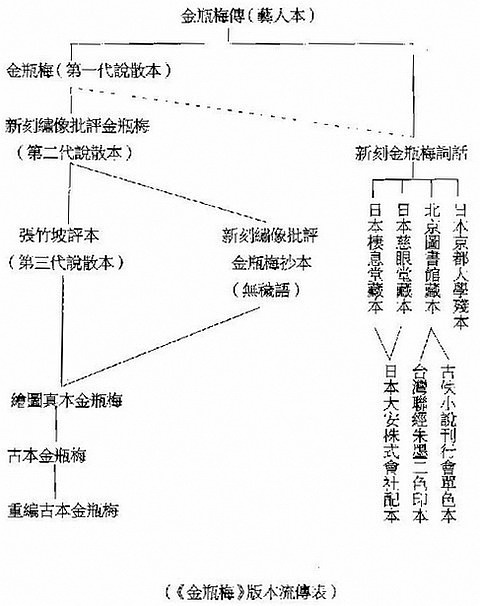
\includegraphics[width=0.6\textwidth]{pingxing.jpg}
\caption{《金瓶梅》版本流传表(平行观点)}
\label{fig:pingxing}
\end{figure}

孙逊在《金瓶梅鉴赏辞典》列的一个更简洁的版本表,如图\ref{fig:sunxun}。
\begin{figure}[htpb]
\centering
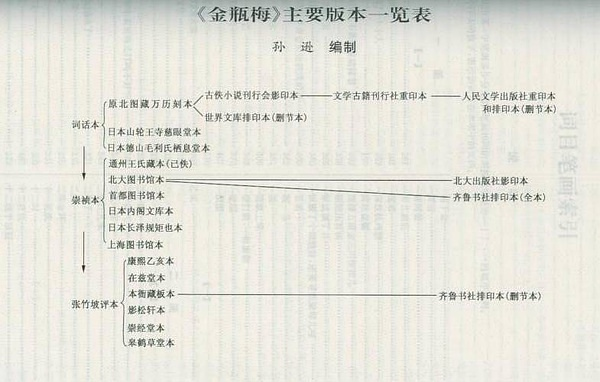
\includegraphics[width=0.8\textwidth]{sunxun.jpg}
\caption{《金瓶梅》版本流传表(孙逊观点)}
\label{fig:sunxun}
\end{figure}


\section{目前出版的主要版本}
以下便对近年来我国出版的金瓶梅的删节本、全本、评注本和整理本等作些介绍\footnote{同上}。

\subsection{洁本}

1985年,在社长兼总编韦君宜女士的果敢主持下,人民文学出版社公开出版了《金瓶梅词话》删节本。这可是建国以来,在公开出版禁书方面的一个突破和创举。稍后,其他出版社也相继出版了洁本以及供内部发行的全本。目前,几乎所有的金瓶梅版本皆已在国内出版,而且,还首次一字未删的出版了崇祯年间刊刻的《绣像金瓶梅》排印本。据笔者所知,近年来先后出版的金瓶梅洁本有以下几种:
\begin{enumerate}
\item 《金瓶梅词话》,人民文学出版社1985年出版。戴鸿森校点,平装三册,首次印1万套,定价12元。有木刻插图36幅,共删19,174字。之后,此一版本曾多次印刷,并由凭证供应改为公开发行。1989年7月还曾出过两卷一套的精装本,附插图35幅,定价55元。
\item 《张竹坡批评第一奇书〈金瓶梅〉》,山东齐鲁书社1987年10月出版。王汝梅、李照煦、于凤树校点。精装两册,附陈全胜绘彩图若干幅。全书共删10,398字,首次印刷1万套,定价28元,后曾多次印刷。甚至有过盗版。
\item 《金瓶梅会校会评本》,中华书局1998年3月出版,内部发行。秦修容校订,系以中华书局所藏清代刊刻的第一奇书为底本。有删节。书后的校勘记中汇总了词话本、崇祯本和张竹坡第一奇书的文字。精装二册,定价268元。
\item 《新刻绣像批评金瓶梅》,浙江古籍出版社1991年8月出版,系该社出版的《李渔全集》的第十二、十三和十四卷,张兵、顾越点校,黄霖审定。删节本,系以现收藏于日本内阁文库的金瓶梅词话为底本。全套《李渔全集》共20册,定价400元。
\item 《词话金瓶梅校注》,岳麓书社1995年8月出版,白维国、卜键校注,系以日本1963年的大安株式会社影印的版本为底本,有删节。全书4册一函,首次印刷3000套。
\item 《新刻绣像批评金瓶梅》,光明日报出版社1997年10月出版,温京华、田军校点,附插图30幅。系该社出版的《竺翁选集》的第五、六、七卷,全书书共删13,812字。全套《竺翁选集》共7册,精装本,印1000部,定价590元。
\item 《金瓶梅词话》,人民文学出版社2000年10月出版,陶慕宁校注,精装二册,另配以插图若干幅。全书共删4300字,首次印刷8000套,售价96元。此版本装帧设计相当美观,校对甚为认真,用纸,印刷均比较考究,删简也比其他洁本为少,乃是几种洁本金瓶梅中,相当值得阅读和收藏的一个版本。
\end{enumerate}

洁本系统表现了当前出版界以及文化界审查的丑态,经过删改的所谓”洁本“《金瓶梅》失去了其文本意义上的完整性,如果有意于认真研读甚至钻研分析,这种”洁本“仅有校勘和利于阅读的意义。虽然删改的性描写对于本书的价值并没有想象中的大,同时其性描写在单纯的文学意义上并不足以撼动本书的思想意义,但删去仍然毁坏了其整体的文学气象。一个现代社会的成年人不会汲汲于本书的性描写,甚至我在读过一半后就对这类性描写感到厌倦,因此其删减并没有什么意义。

\subsection{足本}

   早在1931年,有人在山西介休发现了木刻本《金瓶梅词话》,当时就引起学者和专家的注意。1933年,北京孔德图书馆的马廉先生更集资影印过120部。鲁迅先生和郑振铎先生等皆曾重金订购。建国初期,根据毛泽东主席关于“《金瓶梅》可供参考,就是书中污辱妇女的情节不好,各省委书记,可以看看”的指示,有关部门曾以1933年版为底本影印了2000套(也有印1000套一说)编号登记发行,供省、军级干部及少数文学家购买。因此书供应范围极小,知道的人不多,影响甚小。据了解,国内先后出版过的金瓶梅全本有以下几种:
\begin{enumerate}
\item 《新刻金瓶梅词话》,北京文学古籍刊行社1957年10月出版,线装二函21册,文字20册,图一册,每回两幅,共200幅图,系以1933年影印本为底本,定价40元。这套书曾于1991年4月重印,仍内部发行,每套定价1200元。不过,原书所缺第52回的两页已另行改用日本大安株式会社1963年影印本配补而不再借用崇祯本52回的7、8两页。
\item 《金瓶梅词话》,香港太平书局1982年8月出版,系据1957年版缩尺影印,但将200幅插图分别移到每回之前各两幅。至2000年底,此版本已先后印刷16次,除6册的平装本外,还出过两册一套的精装本。目前,书市上此版本的盗版比较多,几十元便可买到一套。
\item 《新刻绣像批评金瓶梅》,北京大学出版社1988年8月影印,4函36册,印数1000套,每回有插图2幅,内部发行,供副教授以上的文科教员购买,定价700元。
\item 《金瓶梅词话》,香港梦梅馆1988年10月初版,现已出第三版。有线装和平装两种。线装本:梅节校勘,陈少卿钞录。此版本系以日本大安株式会社影印的版本为底本,另以台湾联经出版事业有限公司朱墨二色套印原北京图书馆藏金瓶梅词话为副本,另参考北京大学本和日本内阁文库之新刻绣像批评金瓶梅、在兹堂本和崇祯本之皋鹤堂批评第一奇书金瓶梅等丛多版本,同时,吸收国内、外众专家的研究成果。经梅节先生自1988年来三次精心校点,纠正原书中讹错七千余处,是词话本中相当接近原著和可读性比较高因而颇有参考价值的一种版本。目前,书市上偶有再版铅字印刷本的盗版出售,售价几十元一套。
\item 《新刻绣像批评金瓶梅》,齐鲁书社1989年6月出版,齐烟、王汝梅会校。这部崇祯本的会校本配有插图200幅,印8000套,定价175元。
\item 《皋鹤堂批评第一奇书金瓶梅》,吉林大学出版社1994年10月出版,王汝梅校注。全书2册,印3000套。
\item 《会校会评金瓶梅》,香港天地图书有限公司1998年出版。刘辉、吴敢辑校,平装5册一函。系以北京首都图书馆藏《皋鹤堂批评第一奇书金瓶梅》为底本,另据其他7种有代表性的说散本会校;而评语则收录北京首都图书馆藏《新刻绣像批评金瓶梅》等7种说散本的评语,包括文龙的评语和张竹坡后人家藏本的墨评。附北京大学藏《新刻绣像批评金瓶梅》的刻印精美插图200幅。这套会校会评本是说散本中相当有参考价值的一种版本。原书定价480港币。书市上偶见影印盗版,有的朱墨套色,有的单色,但前者的纸质较差,售价都不大贵。
\end{enumerate}

